\section{Current Challenges and Visions}\label{sec:main}
In the following paragraphs we will go through different challenges that occurred to researchers and the visions they have.

\subsection{Architecture}
As edge computing is extending the boundaries of cloud computing, a lot of concepts and paradigms can be applied to edge computing in an altered way. On top of that, the edge shall become more user-centric and allow an inwards control coming from the edge and not the control from the cloud that has been accepted in recent years with cloud computing.

\subsubsection{Communication}\hspace*{\fill} \\
Taking into account that edge devices come in different sizes and therefore might have limited computational power and battery capacity, communication requires extra consideration to make it efficient.

Edge devices enter a state where they might not be reachable for an uncertain time and cannot, therefore, build up a continuous connection to neither other edge devices nor the cloud.
To counter this weakness peer-to-peer is the most applicable as the basis of edge computing communication. It may has been introduced in 1999 and mostly been associated with illegal activities, but is perfectly capable of scalable and decentralized communication in networks that are physically and logically close-by \cite{GarciaLopez:2015:ECV:2831347.2831354}.

Peer-to-peer is highly tolerant against churn, meaning that a lot of nodes are able to join and leave without drawbacks for the network, which in the case of edge computing is perfect as edge devices can at any point not be reachable for unidentified reasons.

Further on peer-to-peer shall blend together cloud computing and edge computing, by having a stable and decentral communication between edge nodes, but still maintaining a traditional connection to the cloud if additional resources are needed \cite{GarciaLopez:2015:ECV:2831347.2831354}.

\subsubsection{Hybrid Architecture}\hspace*{\fill} \\
This previously mentioned mixture of communication can be used to establish a hybrid architecture. The resources of the edge devices can be complemented with temporary usage of cloud storage services \cite{GarciaLopez:2015:ECV:2831347.2831354} and allow to work at a fraction of traditional cloud computing use cases.

Resources provided by peer-to-peer edge networks can be used to build nano data centers, micro clouds, community clouds or edge clouds \cite{GarciaLopez:2015:ECV:2831347.2831354}. Those soon to be services become more attractive as soon as a global player such as Google, Amazon or Microsoft offer a managed version of these, but also established telecommunications provider are be able to compete with the global players of cloud computing and might even outdo those as they have already a headstarts through their base stations all over the world.

\subsubsection{Microservices and modularity}\hspace*{\fill} \\
\todo{maybe current state of the art? not related to any papers, but might be interesting... mostly been used in context with fog computing, but is applicable to edge computing}

\subsubsection{Latency}\hspace*{\fill} \\
One of the strongest arguments for a change in current computational paradigms is latency. The current centralized cloud computing is not able to keep up with the requirements of real-time applications as depending on where it is hosted and the user is located some delay to the messages has to be added.
Edge computing seems to be the logical next step to be closer to the user and thereby reducing the latency and allowing almost real-time communication with a delay of 25ms to 50ms instead of far above 100ms.

Health emergency, public safety, and autonomous driving are profiting most of edge computing as decisions and quick computing can be done close to the edge rather than collecting information and making a decision in the cloud \cite{7488250}.

\subsubsection{Bandwidth}\hspace*{\fill} \\
Latency is not the only aspect that has to be considered when talking about transmission time. High bandwidth can reduce transmission time and thereby minimizes latency.
As edge devices don’t always have a high bandwidth connection to the cloud but usually a high bandwidth connection in the local network or to a closer node those can be utilized to act as gateway to aggregate the data, do the requested computing and then send the final result to the cloud. If none of the edge devices have enough computational power for the task then at least the data can be aggregated and compressed to save bandwidth compared to the usual rather simple transmission \cite{7488250}.

As a simple example, for facial recognition, the edge devices might not have enough computing power but what can be done is compress and preprocess the picture before it is uploaded, hence the bandwidth reduction.

\subsubsection{Scalability}\hspace*{\fill} \\
A persistent topic in cloud computing, peer-to-peer and therefore edge computing as well has always been scalability.
Whereas cloud computing had consistent problems with scalability and elasticity, and peer-to-peer overcomplicated everything with churn and dynamism, edge computing shifts these challenges towards new topics.

The problems of peer-to-peer might not be hindering that much anymore as stable cloud resources can be used, but a big challenge arises as a tradeoff between computing and communication has to be found \cite{7488250}\cite{GarciaLopez:2015:ECV:2831347.2831354} and which edge one can trust and which one not.

Scalability is an ongoing problem in edge computing as the control is now in the edge, but management has yet to be defined and is most probably gonna end up in the cloud.

The biggest challenge in correlation with scalability is security and finding a proper way to deal with the overhead that is going to be introduced through encryption to provide secure communication between the edge devices and the cloud.

\subsubsection{Dealing with Data Explosion and Network Traffic}\hspace*{\fill} \begin{figure}[h]
    \centering
    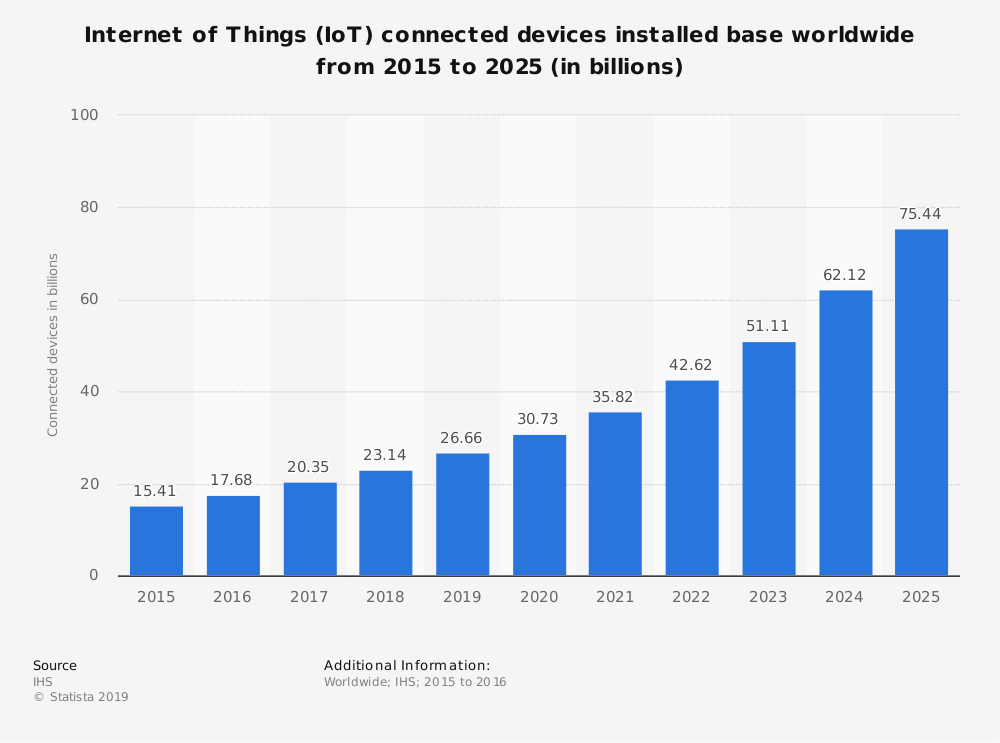
\includegraphics[width=1\textwidth,height=0.8\textwidth]{resources/images/global_iot_devices.png}
    \caption{Forecast of worldwide connected Internet of Things devices}
    \label{fig:global_iot_devices}
\end{figure}

As can be seen in chart \ref{fig:global_iot_devices} the number of IoT connected devices drastically increased over the last years and by 2025 are supposed to be five times the amount of connected devices than 10 years earlier and come to a total of 75 billion IoT devices.

\begin{figure}[H]
    \centering
    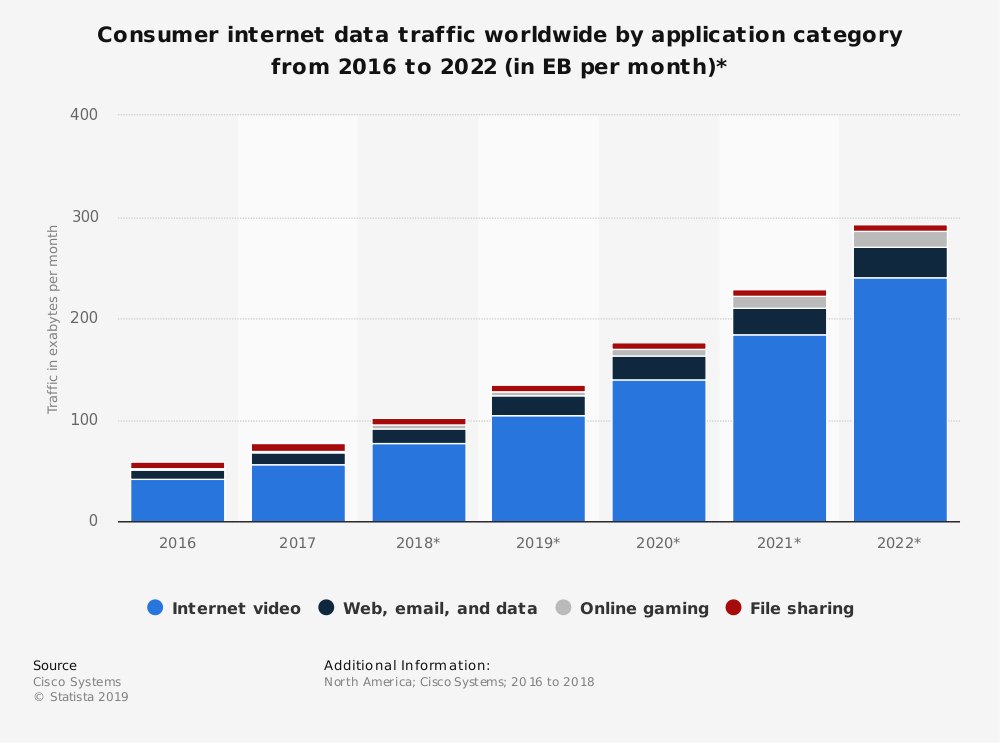
\includegraphics[width=1\textwidth,height=0.8\textwidth]{resources/images/global_traffic.png}
    \caption{Forecast of worldwide internet traffic}
    \label{fig:global_traffic}
\end{figure}

Looking at the internet traffic presented in chart \ref{fig:global_traffic} the total volume of data traffic per month is expected to be doubled within the next 3 years compared to today.

To harness and actually be able to deal with the amount of data and devices edge computing is a good start to a decentralized cloud but won’t be able to handle all of the traffic and computing itself. Fog computing is a good addition to do computing close to the edge where edge devices might not have enough computational power but still need a lower latency compared to an exchange of traffic to the cloud \cite{7796149}.

\subsection{Privacy \& Security}
Privacy and security are both aspects that are thought to be lost with cloud computing and that might be true for the beginning of the cloud era but nowadays a lot of standards got established to ensure a secure connection. Privacy in the cloud remains a highly doubtable concept. Hence, privacy and security are the most important services that should be provided \cite{GarciaLopez:2015:ECV:2831347.2831354}.

\subsubsection{Personal Space in the Edge}\hspace*{\fill} \\
The first out of the three visions regarding privacy in the edge.
Edge computing brings back trust and control to the user about their data. The idea is that the user keeps their own so-called information silo and has full control over it, meaning they are able to share specific information with third-party applications or users and the full control stays at the user.
A new architecture has to be established with a focus on privacy-aware data sharing and advanced access control mechanisms \cite{GarciaLopez:2015:ECV:2831347.2831354}.
The paradoxical is the suggestion to use the cloud to host the information silos together with encryption and privacy guarantees.

\subsubsection{Social Space in the Edge}\hspace*{\fill} \\
The current established online social networks such as Facebook and Linkedin are based on a centralized model with a centralized database where only the company itself has full access to and makes money based on the users’ data through advertising for example.

Approaches such as Diaspora or Mastodon are decentralized social networks that give the control over data back to the user, as long as the user hosts their own server, which for most people is not feasible.

In close proximity technologies such as Bluetooth or Wifi Direct shall be used to establish a link to other edge devices and allow close-by communication paired with connections to resources at the edge or cloud depending on the the tradeoffs of computing and battery consumption. Altogether this allows an interesting use case of online social networks without the need to setup a server.

While those novel online social networks are interesting for deep social mining as none of those instances are centralized, recommender systems are going to deeply suffer on the lack of information that was previously provided through centralized databases.

\subsubsection{Public Spaces in the Edge}\hspace*{\fill} \\
The last of the three visions is public space in the edge and is also the more challenging and complicated vision.

Every person automatically participates as soon as they own a mobile device or sensor e.g. smartwatch and switches between different services providers with different definitions of privacy and security.
One challenge will be that when the user moves in the public space they are going to generate a track of information that can potentially expose the user and edge technologies are going to have to take care of this to provide a guarantee of confidentially and security.

Currently, there are different research approaches on how to deal with trust in the public space. As everyone is supposed to be an active participant rather than a passive one trust has to be somehow established between the different participants including sensors.
One of the approaches is a reputation system or an overall anonymous communication between the participants.

\subsubsection{Edge Computing as a Service}\hspace*{\fill} \\
In recent years managed cloud services became the norm and allows companies to efficiently provision and release computational resources on the go.

Such services need to be provided for edge computing together with a service level agreement (SLA).
One common aspect of cloud computing is multi-tenancy, where security is a prime concern for edge devices.

Containers are the go-to for running applications in an abstracted but efficient form and are thereby also perfectly suitable for edge computing but need to be more robust. Perfect additions for containers are either gvisor or kata containers, which both provide a secure layer between hardware and application.

Traffic, energy, and maintenance cost have to be taken into account depending on data location.

\subsubsection{Security}\hspace*{\fill} \\
The current work done on cloud security can be taken into account as a starting point for edge computing e.g. encrypted data stores, queries over encrypted data or secure end-to-end communication.

Edge computing has to consider the existence of malicious nodes paired with trusted nodes on the same network and remains an open challenge on how to properly deal with it.
One way would be to introduce secure routing between participants, but even this might not be enough to protect from a man in the middle attack or a trusted node turning rogue. Similar problems apply to a chain of trust.

With a decentralized system, data fragmentation is inevitable and has to be properly dealt with, meaning secure encryption of those fragments has to be provided.

Important is that every additional layer of security and privacy is going to add additional constraints on the computational resources and might make some edge devices not usable for certain use cases.